% Document type with options
\documentclass[fleqn,letterpaper,12pt]{report}

% Required packages and settings (DO NOT UPDATE THIS)
\usepackage{UN5390}
../LaTeXTemplates/Course/UN5390_Settings.tex

% Assignment-specific setting (UPDATE THIS WHEN NECESSARY)
\week{12}

% Document begins
\begin{document}

% Title (DO NOT UPDATE THIS)
\assignmenttitle

%
\phantomsection
\addcontentsline{toc}{section}{Problem \# 1}
\problem
The below is the list of the top ten powerful supercomputers as per the 48th edition of the TOP500 list released in November 2016 \cite{SC16}. The list shows China and the United States competing against each other in the field of supercomputing.
\begin{table}[h!]
\centering
\caption{Top 10 most powerful supercomputers, SC16, November, 2016}
\label{my-label}
\scalebox{0.85}{
\begin{tabular}{l|l|l|r|r|r|r}
	\multicolumn 4 {c}{} &
	\multicolumn 2 {|c|}{\bf{TFLOPS}}&
	\multicolumn 1 {c}{}\\ \hline
 \bf{\#} & \bf{Name}            & \bf{Location}         &\bf{Processors}&\bf{Expt} &\bf{Theory} &\bf{Power(MW)}\\ 
 \hline 
 1  & Sunway TaihuLight         & 2016, NSCW, China      & 10,649,600   & 93,014.6  & 125,435.9 & 15.371 \\
 \hline
 2  & Tianhe-2                  & 2013, NSCG, China      & 3,120,000    & 33,862.7  & 54,902.4  & 17.808 \\
 \hline
 3  & Titan                     & 2012, ORNL, USA        & 560,640      & 17,590.0  & 27,112.5  & 8.209 \\
 \hline
 4  & Sequoia					& 2012, LLNL, USA		  & 1,572,864   & 17,173.2  & 20,132.7  & 7.890 \\
 \hline
 5  & Cori 						& 2016, LBNL, USA		  & 622,336		& 14,014.7  & 27,880.7  & 3.939 \\
 \hline
 6  & Oakforest-PACS			& 2016, JCAHPC, Japan    & 556,104      & 13,554.6  & 24,913.5   & 2.719 \\
 \hline
 7  & K				     		& 2011, RIKEN, Japan	 & 705,024		& 10,510.0  & 11,280.4  & 12.660 \\
 \hline
 8  & Piz Daint				    & 2012, CSCS, Switzerland& 206,720      & 9779.0	& 15,988.0  & 1,312 \\
 \hline
 9  & Mira		   			    & 2012, ANL, USA		 & 786,432	    & 8,586.6	& 10,066.3  & 3.945 \\
 \hline
 10 & Trinity				    & 2015, LANL, USA        & 301,056		& 8,100.9   & 11,078.9	& 4.233 \\
 \hline
\end{tabular}%
}
\end{table}
%
\\
Titan is known for being the first major supercomputer that uses a hybrid architecture, that utilizes both conventional AMD Opteron CPU's and NVIDIA Tesla GPU accelerators \cite{titan}. It is built using 18,688 compute nodes and handles a total of 38 GB of memory per node. The machine built by Cray at the US government's Oak Ridge National Laboratory (ORNL) with a cost of about 97 million USD. It is being used for projects such as modelling of the molecular physics of combustion, simulating interactions between electrons and atoms in magnetic materials, simulating nuclear reactions with the aim of reducing nuclear waste, simulating galaxies etc.

Clocking in at 16.32 sustained PFLOPs (quadrillion floating point operations per second), Sequoia ranks 4th in the Top500 list of the world's fastest supercomputers released November, 2016. A 96-rack IBM Blue Gene/Q system, Sequoia is enabling modellings that explore phenomena at extreme resolutions. It is built out of 98,304 compute nodes, 1.6 million cores, and 1.6 PB of memory. Sequoia is dedicated to National Nuclear Security Adminstration, NNSA's Advanced Simulation and Computing (ASC) program for stewardship of the nation's nuclear weapons stockpile, a joint effort from LLNL and SNL. The NNSA/LLNL/IBM partnership has produced six HPC systems that have been ranked among the world's most powerful computers so far \cite{sequoia}. 
\newpage
\phantomsection
\addcontentsline{toc}{section}{Problem \# 2}
\problem
The current computing infrastructure includes access to a HPC cluster with 1024 processors with 4 GB RAM per processor, 56 Gbps InfiniBand network and 64 TB archival quality storage. The overall RAM available is 4096 GB. Considering the new donation towards the research, we now have a 8192 processors and each processor is equipped with a RAM of 16 GB contributing towards a total RAM of $\approx$ 131.1 TB. Assuming that the problem is still equally scalable, our total RAM has increased 32 times. Although the calculated RAM is $\approx$ 32 times more, the RAM per core is only 4 GB where as the new machine's RAM per core is 16 GB. So, the increase in per core RAM is almost 4 GB per core. 

Considering the same number of $\tt{FLOPs/CPU \; cycle}$ we observe that the newly donated machine is $\approx$ 8 times faster than the present machine. If the research problem is equally scalable, we see that, the new machine can therefore finish a whole run or equivalently we can solve a problem of size $8N$ in $t$ considering again that the problem is equally scalable.

The ultimate question to answer is whether to solve a problem of size $N$ in 1/8 th of the time $t$ or size $8N$ in $t$ time or sometime in between. This question is equivalent to whether to go for more speed or more parallelism. If the time $t$ is relatively small and saving anymore time is not considered anymore efficient, there would be no reason to make it any further faster. In general sense if the application includes what we call \emph{data parallelism}, it is a simple task to achieve speedup. 

The reasons for whether or not to choose a machine with higher number of processors is purely dependent on :-
\begin{enumerate}
\item time $t$ 
\item amount of parallelism 
\item cost 
\item power
\end{enumerate}
If we have increased performance in terms of time to solve the problem, it might seem reasonable at first to opt for a machine with higher capabilties but a better time is related to the amount of parallelism in the application. Here we consider that the scalabilty is 100\%, so the performance would increase well but $t$ is given to be 90 days so each run  would take 90 days and all the 4 runs would take 360 days which is 360 x 24 x 1024 CPU hours or $\approx$ 1 year time. If we are to use the new machine it would take 40 days which is 40 x 24 x 8192 CPU hours to complete the problem, if we use the new machine we would save ~100,000 CPU hours which is a lot of money.  Because all the costs are covered, it would seem resonable to solve the problem of the same size $N$. 

Now if we look at the total CPU hours and if we are to increase the problem size 8 times, that is $8N$, and if we calculate the CPU hours, then, number of CPU hours on the original machine is 8 x 360 x 24 x 1024 for all the four runs which is 70,778,880 CPU hours. Number of CPU hours on the new machine is 8 x 40 x 24 x 8192 for all the four runs which is 62,914,560 CPU hours, thus we save a total of $\approx$ 8,000,000 Hours.

The only question that remains is that of energy efficiency we know that as the frequency increases the power consumption increases in cubical powers. Since the overall power cost and everything is covered by our generous donor, we can therefore at this point say that it is clearly more profitable and time efficient to solve a problem of size $8N$ in around the same time that might take to solve a problem of size $N$. 
%
\begin{table}[h!]
\centering
\caption{Comparison in terms of CPU hours for all the four runs}
\label{my-label}
\scalebox{1}{
\begin{tabular}{|l|r|r|r|}
	 \hline
           & Original Machine       & New Machine              &   \\

 \bf{Size} & \bf{CPU hours}         &\bf{CPU hours}          &   \bf{Saved CPU hours} \\\hline
     $N$   &    8,847,360			& 7,864,320				   &   983,040	 \\ \hline
	 $8N$  &    70,778,880			& 62,914,560			   &   7,864,320 \\ \hline
 
\end{tabular}%
}
\end{table}
%
If we are to use the machine 8 times in a row, we would save a total of 7,864,320. That being said, the entire problem now comes down to parallelism as discussed earlier. We would obviously go for a larger problem if it has more paraellism in it. If there is not so much thread level parallelism in the problem, we would choose the $8N$ sized problem, if the problem is equally scalable \cite{PK}. 

If there is no risk of losing the job, we could use the resources as required but the other question is about the responsible use of resources \cite{cdresources}. In order to keep the donor happy, the benefitor might have to be resonable and responsible in order to maintain the good will and for potential future funding.

\newpage
\phantomsection
\addcontentsline{toc}{section}{Problem \# 3}
\problem
By intuition as the number of processors that are being used to solve the program are increased, the time of execution should decrease eventually. This is true but if the problem is too small for a single processor there is only an increased lag when we run them on 2 (or more) processors. Therefore, the time of execution is not always inversely propotional to the number of processors that the problem is solved upon.

The for loops in {\tt\textcolor{Green}{matrix\_multiply\_p.m}} is run on number of processors (NPROC) from 1..to..12 using MATLAB's {\tt parfor}. we see that the performance in terms of time of execution increases as processors increase to 2 (and also 3 in case of N = 128) but after that the time of execution increases. This is because as the problem size decreases, the time to fork and join the threads dominates the actual times of execution on each processor. 

\begin{figure}[htbp]
	\centering
	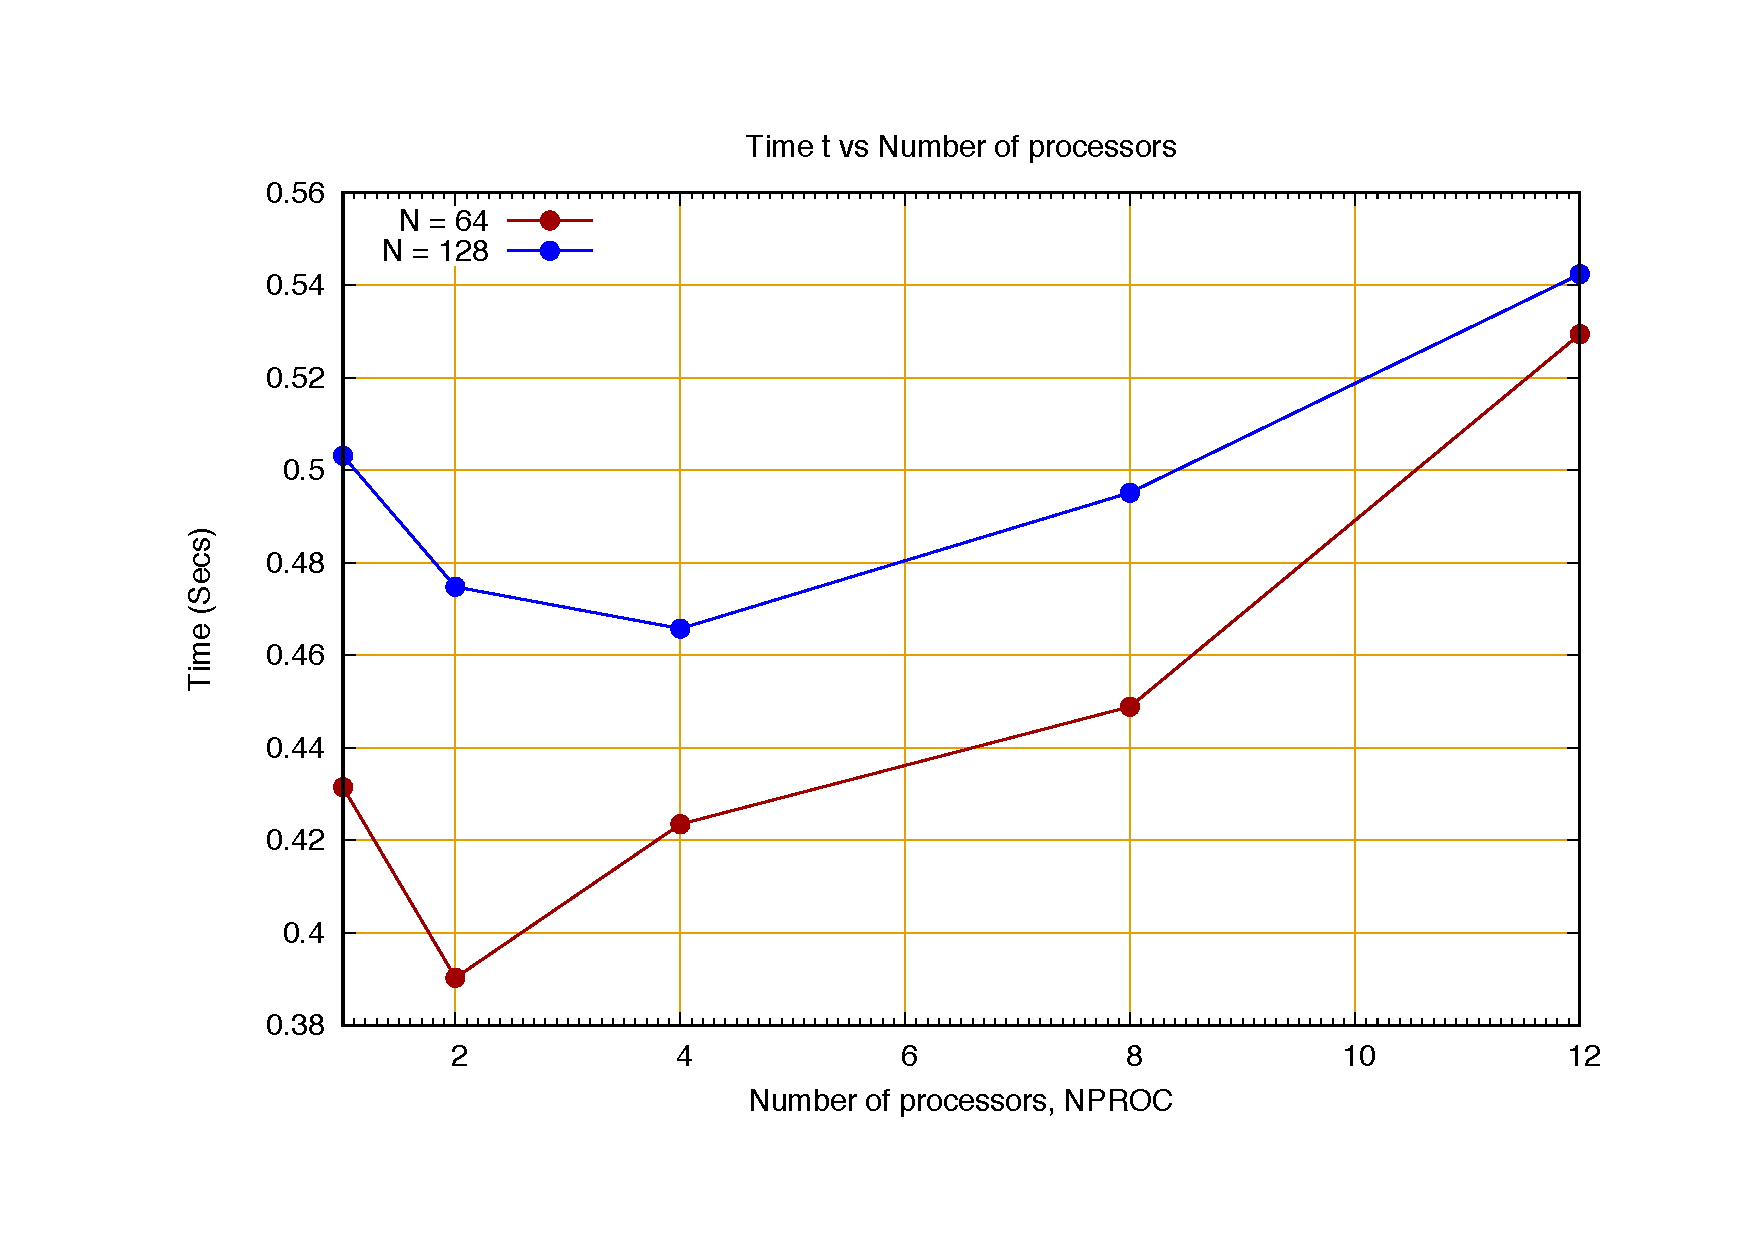
\includegraphics[height=120mm,width=160mm]{64n128.pdf}
	\caption{Times of execution vs NPROC for N = 64 and 128\label{overflow}}
\end{figure}

This tradeoff between time of execution and NPROC should be considered when using more number of processors. It was possible to run the problems only upto NPROC = 8 as the cluster has the {\tt{NumWorkers}} property set to allow a maximum of 12 workers. Therefore NPROC = 16 is not taken into account in doing the analysis \cite{PK}.

The scaled speedups can be plotted as the following. 
\begin{figure}[htbp]
	\centering
	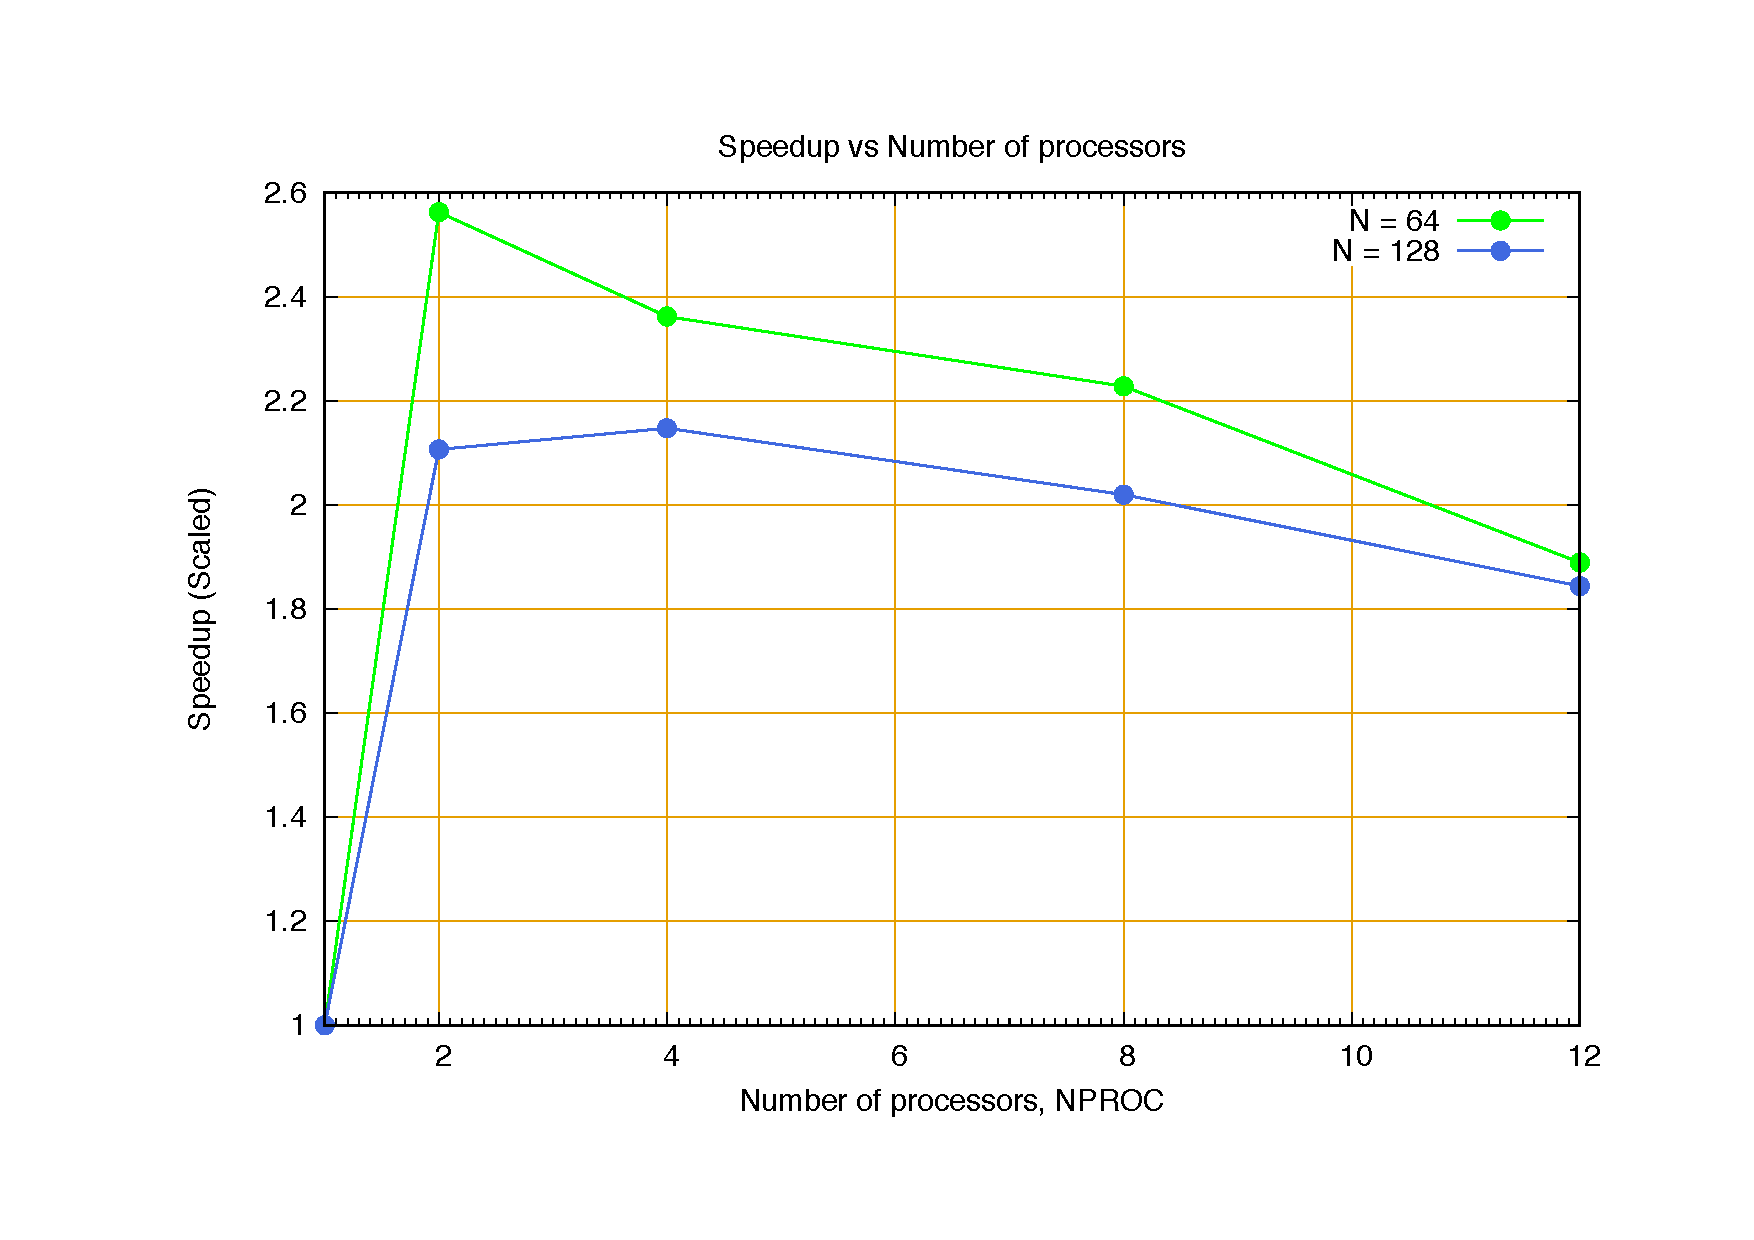
\includegraphics[height=120mm,width=160mm]{64128smat.pdf}
	\caption{Speedup vs NPROC for N = 64 and 128\label{overflow}}
\end{figure}

We see that after a certain point the time of executions increase as NPROC increases where distribution of work and organising results from each processor takes more time than the actual work done each processor. But as the size of the problem increases we see that the forking and joining time is far less when compared to the time saved by utilising multiple processors and therefore the time of execution significantly decreases.
\newpage
We see that as the problem size increases, the speedup starts to become somewhat linear. This can be seen clearly when the size of problem is increased to N = 512.

\begin{figure}[htbp]
	\centering
	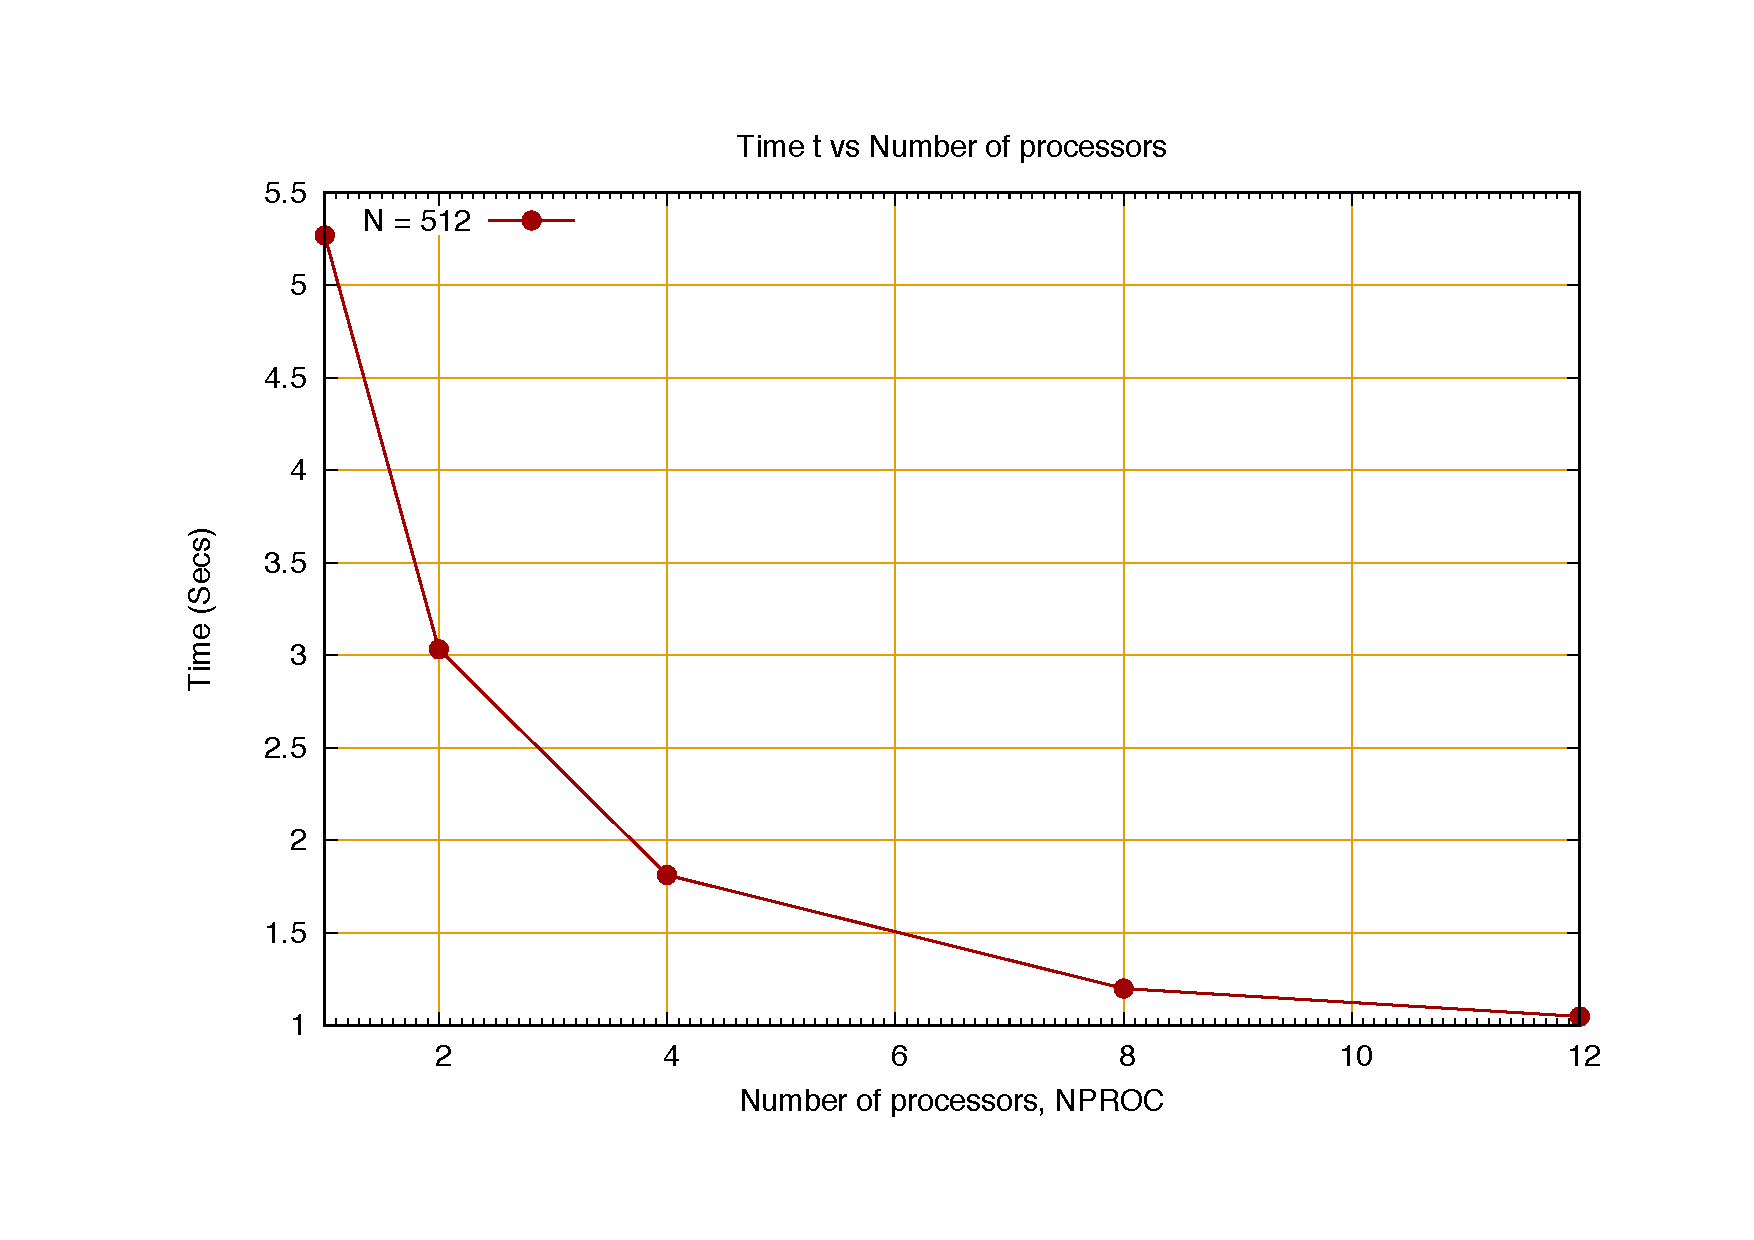
\includegraphics[height=120mm,width=160mm]{512.pdf}
	\caption{Times of execution vs NPROC for N = 512\label{overflow}}
\end{figure}
The physical reason behind this is the time it takes for an electrical signal to traverse a circuit is limited by the speed of light. This is a hard limit, and there is no known way around it. At gigahertz-clocks, we are approaching this limit. However, we are not there yet. 1 GHz means one nanosecond per clock tick. In that time, light can travel 30cm. At 10 GHz, light can travel 3cm. A single CPU core is about 5mm wide, so we will run into these issues somewhere past 10 GHz.
\newpage
The scaled speedup starts to be more relevant to the processor count. This can be further seen when N = 1024. The times of executions significantly decrease with increase in more processors.
\begin{figure}[htbp]
	\centering
	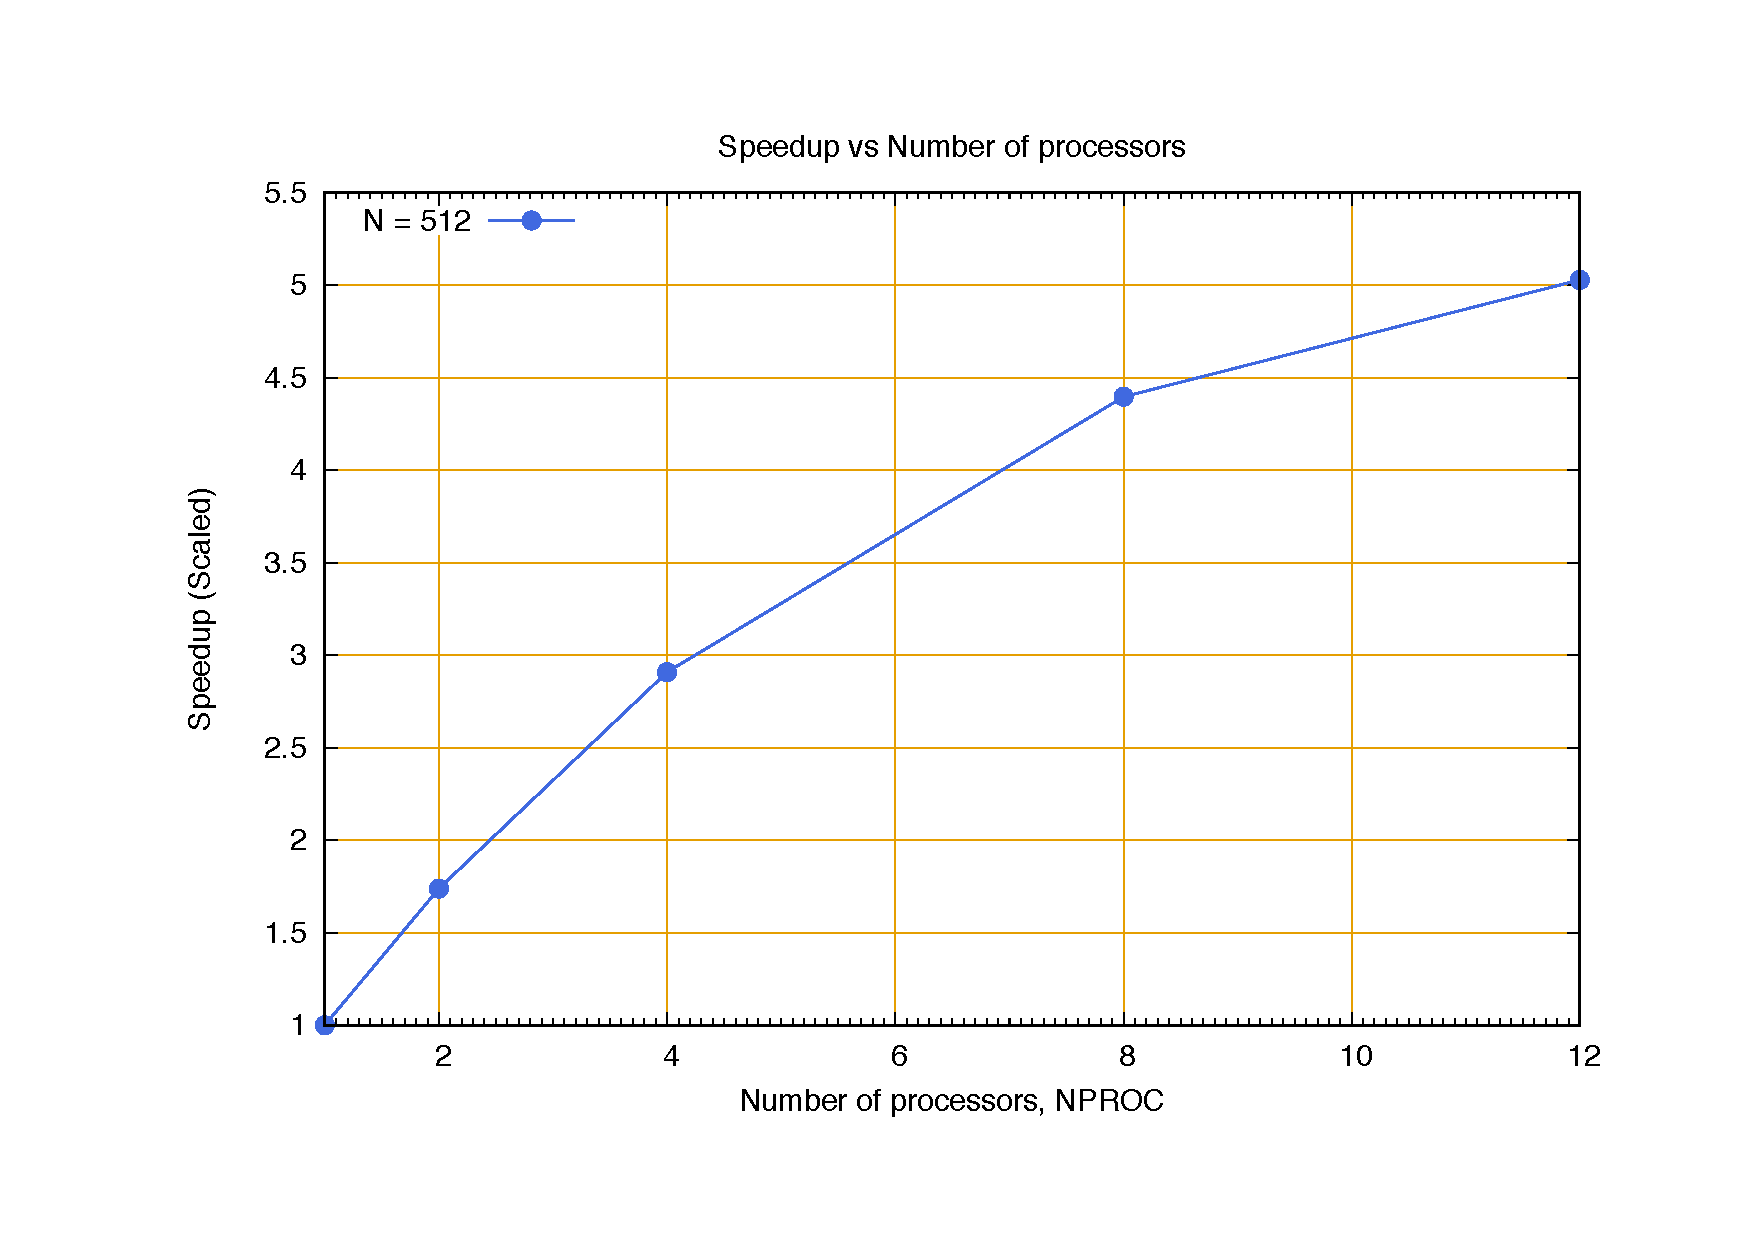
\includegraphics[height=120mm,width=160mm]{512smat.pdf}
	\caption{Speedup vs NPROC for N = 512\label{overflow}}
\end{figure}
So, for example, a 1.5 Ghz dual core CPU may offer performance equal to a 2.0 Ghz single core CPU, but with lower power requirement and less heat generation. This is particularly important in tablet and smartphone design. This is because the frequency or the power comsumed by the CPU is directly proportional to the cubical power of the CPU clock frequency.
\newpage
As NPROC increases, we see a significant decrease in the execution times. The scaled speedup is almost linear. The larger the the size of the problem, the more linear the speedup becomes as each processor is getting a larger dividend of work that its contributing towards which in turn contributes to the overall performance. 
\begin{figure}[htbp]
	\centering
	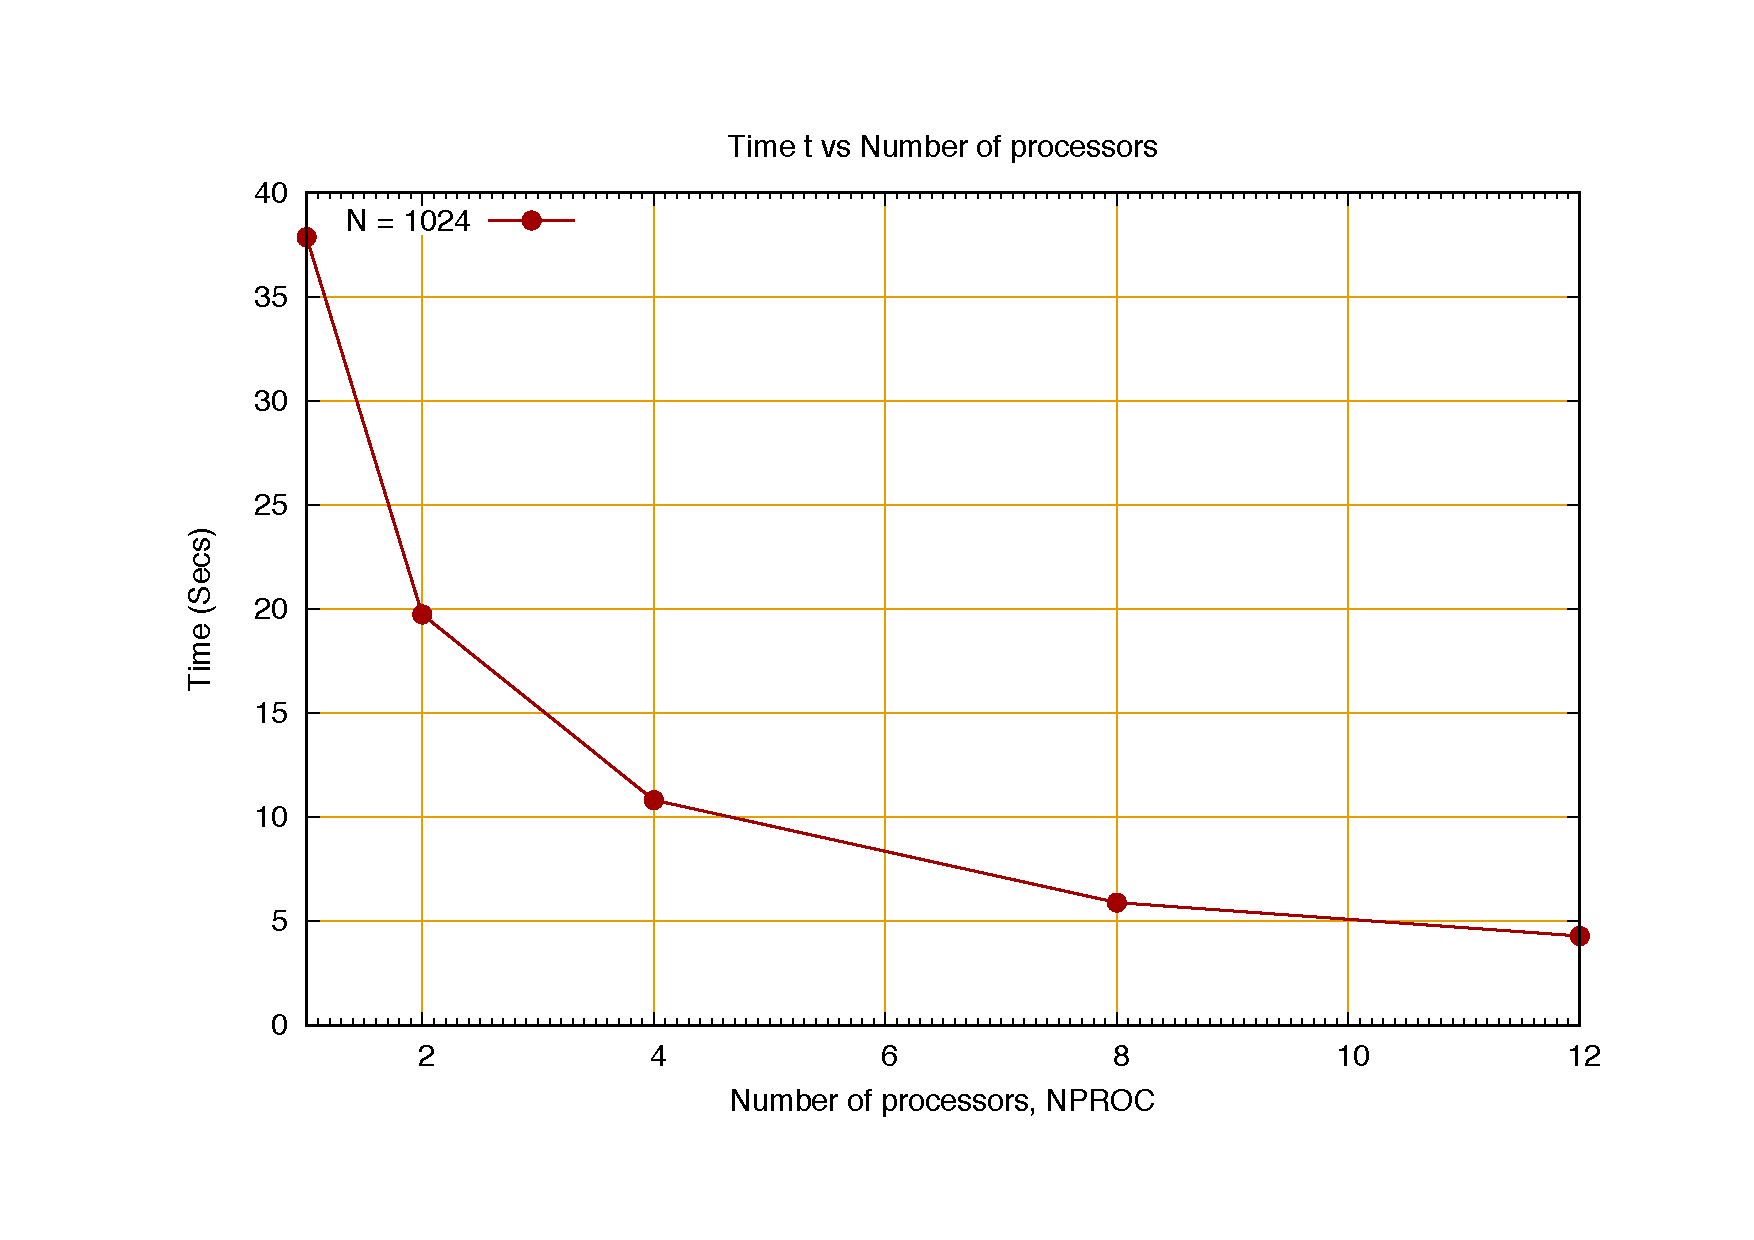
\includegraphics[height=120mm,width=160mm]{1024.pdf}
	\caption{Times of execution vs NPROC for N = 1024\label{overflow}}
\end{figure}

The results can be further increased if we could sum or combine the results on the fly as each processor finishes working on it.
\newpage
The scaled speedups tend to be almost linear when the program size becomes 1024.
\begin{figure}[htbp]
	\centering
	\includegraphics[height=120mm,width=160mm]{1024512smat.pdf}
	\caption{Speedup vs NPROC for N = 512 and 1024\label{overflow}}
\end{figure}

Thus, the above examples show that the tradeoff between the number of processors and the size of problem is a very important factor not only for efficiency of the program but also for efficient use of the resources. The program is in the file {\tt\textcolor{Green}{matrix\_multiply\_p.m}}. As we come up with ways to utilise the processors efficiently or device algorithms that go well with the processors, we can improve the performance on multicores.
\vfill

\newpage
% References
% http://tex.stackexchange.com/questions/84099/bibliographies-from-multiple-bib-files
\phantomsection
\addcontentsline{toc}{section}{References}
\section*{References}
\bibliographystyle{unsrt}
\bibliography{sgowtham,slanka} % REPLACE john WITH YOUR MICHIGAN TECH ISO USERNAME

% Document ends
\end{document}
